\subsection{Motivation}

\begin{frame}{~}
	this notation is already nice for communication, but semantics matter (for large models, it does not suffice to look sharply)

	why is this needed? (forward ref?)

	this section shall teach the relationship between FMs and formulas and FMs and sets (i.e., Damiani 2020, Batory 2005), so: FM semantics

	also, (valid) total configurations should be explained here (how a computer can check them, this can be checked easily when an FM is encoded eg as runtime variability, but all other SAT-based questions are hard to answer)

	recount the example model here
\end{frame}

\subsection{List of Valid Configurations}

\begin{frame}{~}
	what is a (valid) configuration? define as a set of selected features (only later extend to partial configurations)

	this is basically an Excel sheet

	first explain product lists / sets and configuration validity (ie, set membership): (use same example)

	$ext-sem (FM) = \{ C \mid C in 2^F | C satisfies all FM rules \}$

	this is a nice (readable) semantics (directly connected to relational databases) but impractical to check, so we need formulas as a concise representation
\end{frame}

\subsection{Universal Variability Language}

\subsection{Propositional Formulas}

\begin{frame}{~}
	Syntax of formulas

	explain $\pand, \por, \pnot, \pimplies, \pequals$

	here, we do not allow $\forall, \exists$ (extensions exist: QBF (e.g., slicing), FOL (non-Boolean models))
\end{frame}

\begin{frame}{~}
	show running example as a formula
	
	explain intuition behind elements of formula

	motivate very shortly why this might be nice

	there is evidence (Knueppel) that the full expressive power of Boolean formulas is needed for real-world formulas
\end{frame}

\subsection{From Diagram to Formula}

\begin{frame}{-- Algorithm}
	formal algorithm for transformation into FOL (and then CNF?)
\end{frame}

\subsection{Canonical Formula Representation(s?)}

\begin{frame}{-- Conjunctive Normal Form}
	CNF is a universal language for saving Boolean formulas, maybe explain it here?
\end{frame}

\begin{frame}{-- Equivalent Transformation}
	
\end{frame}

\begin{frame}{-- DIMACS File Format}
	
\end{frame}

%(state BDD?)
% probably not - (knowledge compilation: there are many nuances between CNF and BDD, maybe discuss?)

\subsection{Other Representations} %variations? these are not only other representations of the same notation

\begin{frame}{~}
	Extended Feature Models
	
	%at the end (what else is there?): in practice, we also have non-Boolean features/attributes/constraints over attributes (more details on efficiency in third block)

	Cardinalities

	Linux/Kconfig % tri-state features
\end{frame}







% put in second block
\subsection{Enumerating All Configurations}
\begin{frame}{\insertsubsection}
	\leftandright{
		%\myexampletight{}{\centering\includegraphics[width=.75\textwidth]{db-constraint}}
		\myexample{26 Valid Configurations}{
			\footnotesize
			\leftandright{
				$\{B,G,W\}$\\
				$\{B,P,W\}$\\
				$\{B,G,P,W\}$\\
				$\{B,D,W\}$\\
				$\{B,G,D,W\}$\\
				$\{B,P,D,W\}$\\
				$\{B,G,P,D,W\}$\\
				$\{B,P,T,W\}$\\
				$\{B,G,P,T,W\}$\\
				$\{B,D,T,W\}$\\
				$\{B,G,D,T,W\}$\\
				$\{B,P,D,T,W\}$\\
				$\{B,G,P,D,T,W\}$
			}{
				$\{B,G,U\}$\\
				$\{B,P,U\}$\\
				$\{B,G,P,U\}$\\
				$\{B,D,U\}$\\
				$\{B,G,D,U\}$\\
				$\{B,P,D,U\}$\\
				$\{B,G,P,D,U\}$\\
				$\{B,P,T,U\}$\\
				$\{B,G,P,T,U\}$\\
				$\{B,D,T,U\}$\\
				$\{B,G,D,T,U\}$\\
				$\{B,P,D,T,U\}$\\
				$\{B,G,P,D,T,U\}$
			}
		}
	}{}
\end{frame}

% \subsection{Linux Feature Model}
% \begin{frame}{\insertsubsection}
% 	\vspace{28mm}~\hspace{-15mm}\href{https://dl.acm.org/doi/abs/10.1145/3382025.3414943}{\includegraphics[width=1.2\linewidth,trim=100 510 100 170,clip]{linux-bdd}}
% \end{frame}

\subsection{Dependencies Modeled in Excel}
\begin{frame}{\insertsubsection}
	\vspace{-7mm}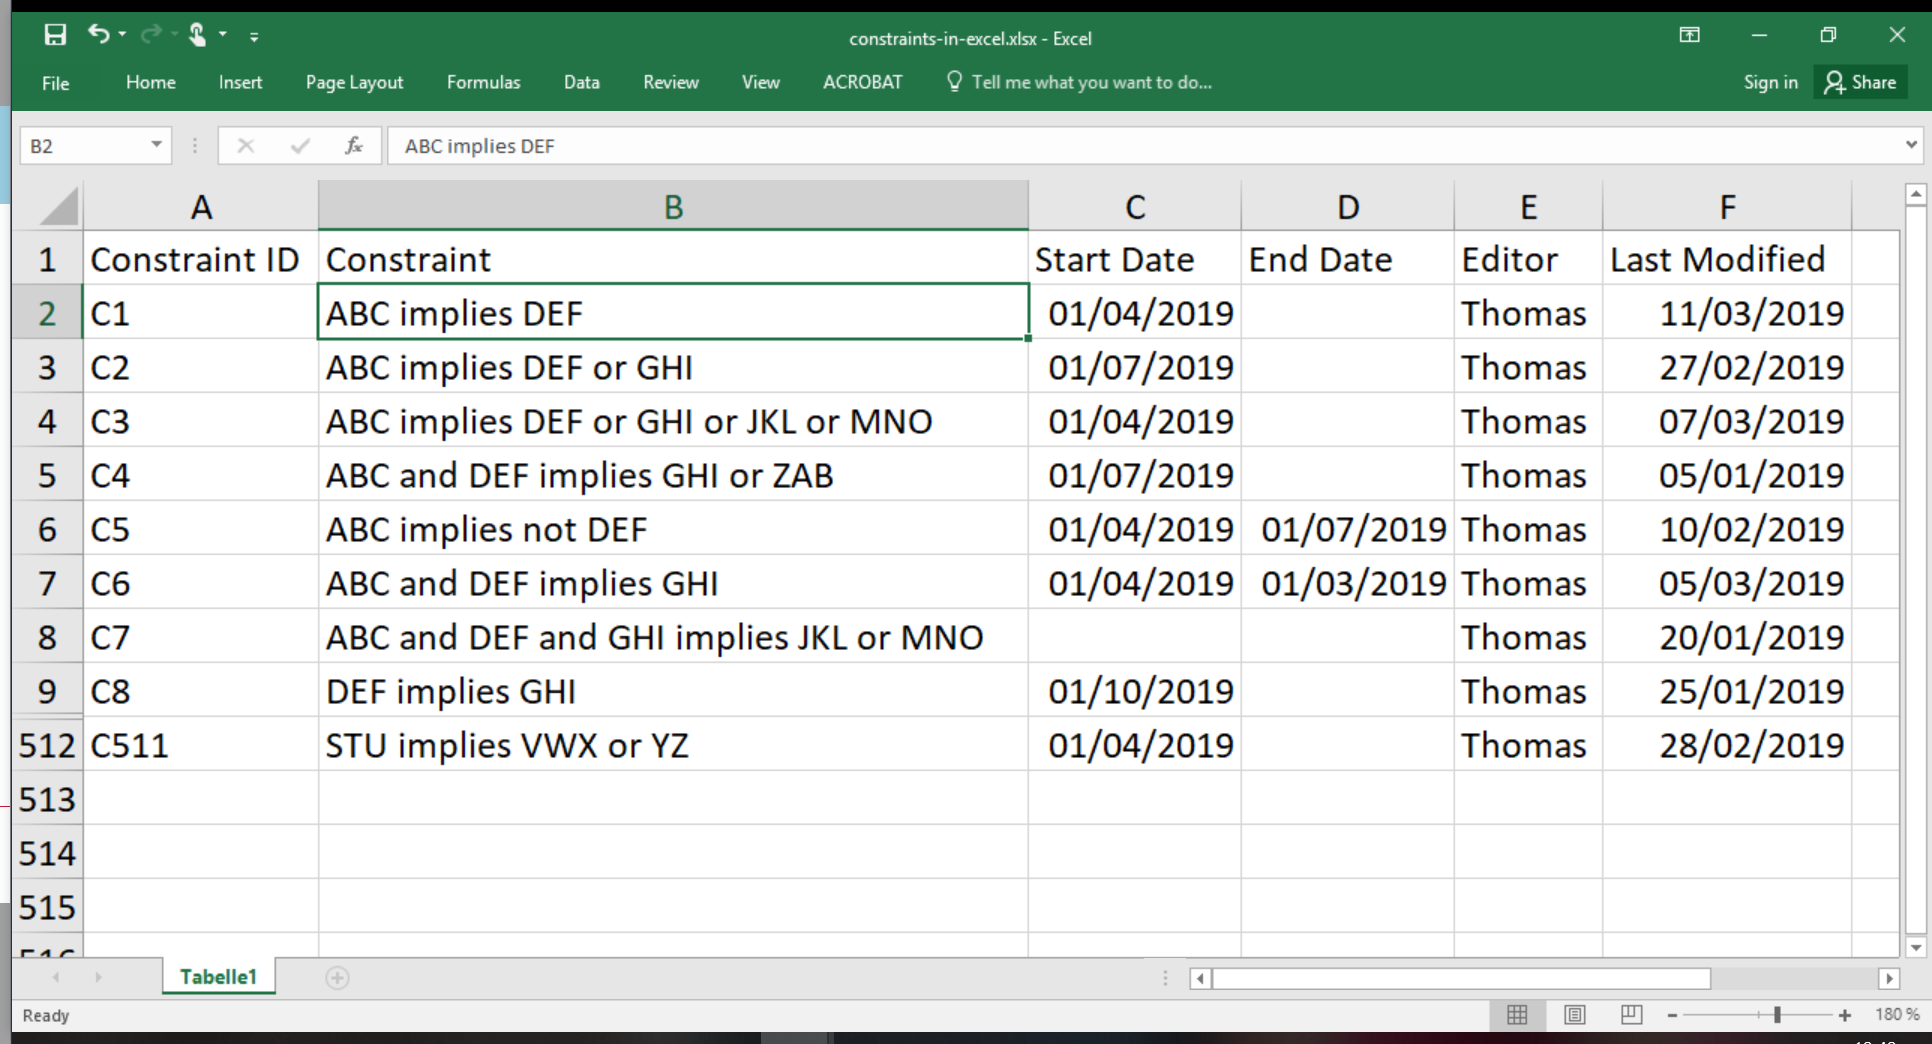
\includegraphics[width=.7\linewidth,trim=10 10 0 10,clip]{constraints-in-excel}
\end{frame}